\documentclass[tikz,border=6pt]{standalone}
\usepackage[T1]{fontenc}
\usepackage[utf8]{inputenc}
\usepackage{tikz}
\usetikzlibrary{automata,positioning,arrows.meta}
\tikzset{>=Stealth,every state/.style={minimum size=9mm,inner sep=1pt,font=\small}}
\begin{document}
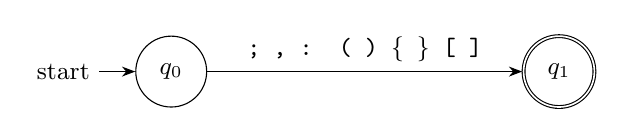
\begin{tikzpicture}[->,node distance=40mm,font=\small]
  \node[state,initial] (q0) {$q_0$};
  \node[state,accepting,right=of q0] (q1) {$q_1$};
  \path (q0) edge node[above] {\texttt{; , : ( ) \{ \} [ ]}} (q1);
\end{tikzpicture}
\end{document}
